\begin{figure*}[t] \centering
    \makebox[0.33\textwidth]{\footnotesize Input A}
    \makebox[0.33\textwidth]{\footnotesize Input B}
    \makebox[0.33\textwidth]{\footnotesize Input C}
    \\
    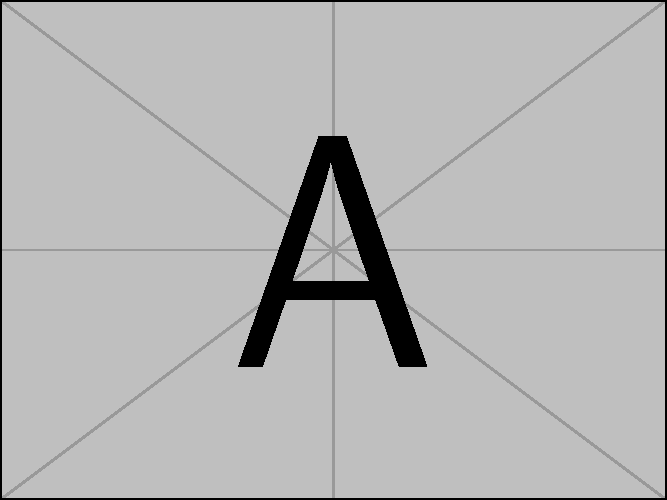
\includegraphics[width=0.33\textwidth]{example-image-a}
    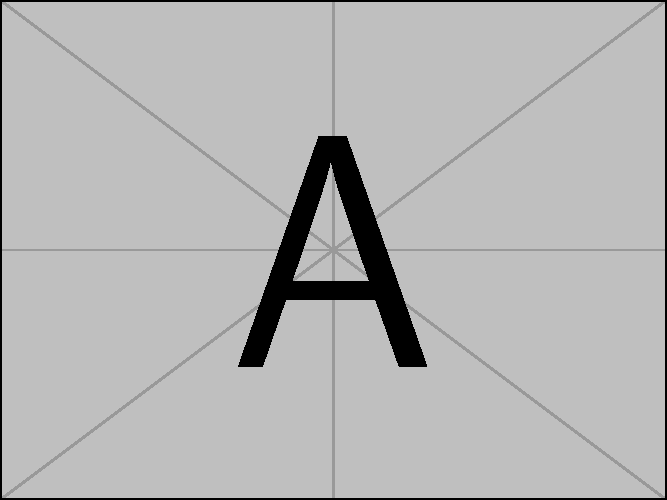
\includegraphics[width=0.33\textwidth]{example-image-a}
    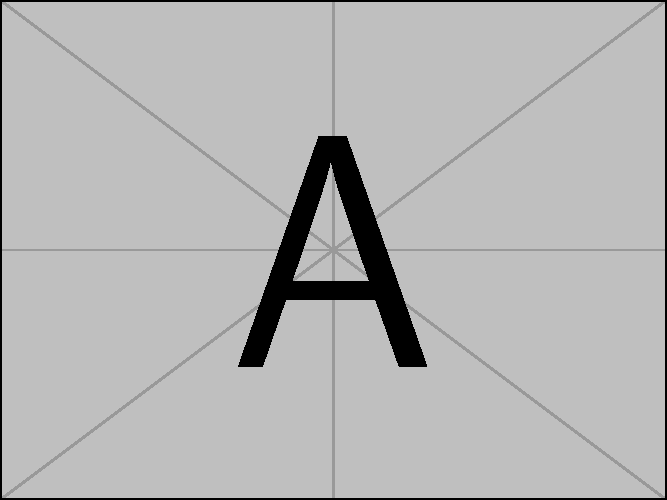
\includegraphics[width=0.33\textwidth]{example-image-a}
    \\
    \makebox[0.495\textwidth]{\footnotesize Overlapped Input} \hfill
    \makebox[0.495\textwidth]{\footnotesize Our Result}
    \\
    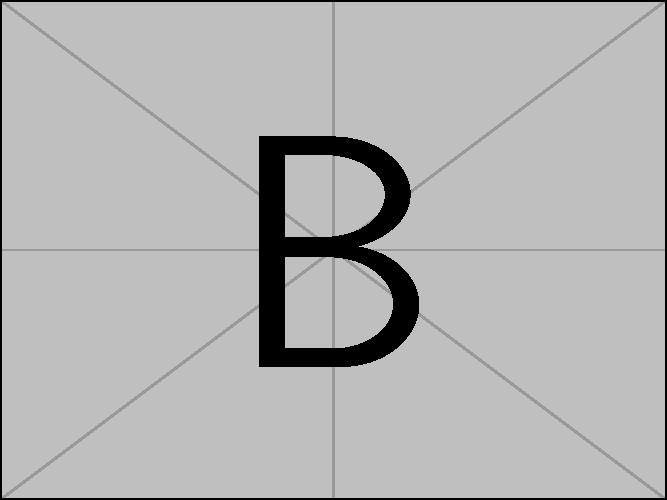
\includegraphics[width=0.495\textwidth]{example-image-b} \hfill
    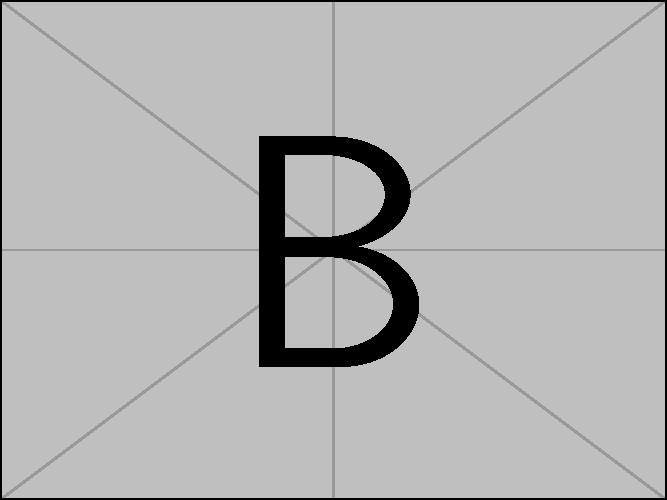
\includegraphics[width=0.495\textwidth]{example-image-b}
    \\
    \makebox[0.162\textwidth]{\footnotesize Method A}
    \makebox[0.162\textwidth]{\footnotesize Method B}
    \makebox[0.162\textwidth]{\footnotesize Method C}
    \makebox[0.162\textwidth]{\footnotesize Method D}
    \makebox[0.162\textwidth]{\footnotesize Method E}
    \makebox[0.162\textwidth]{\footnotesize Method F}
    \\
    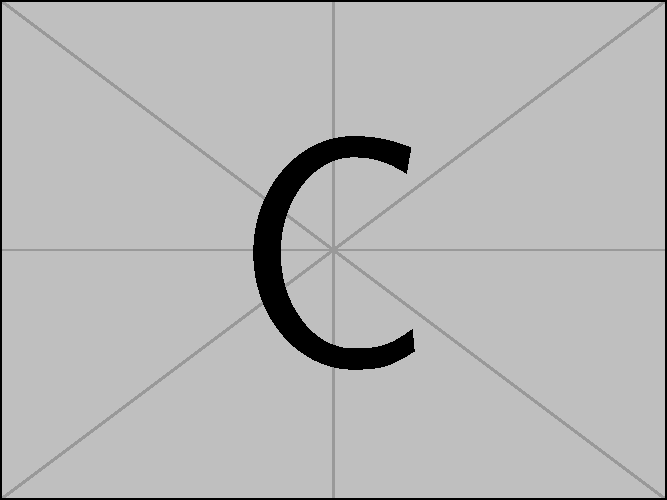
\includegraphics[width=0.162\textwidth]{example-image-c}
    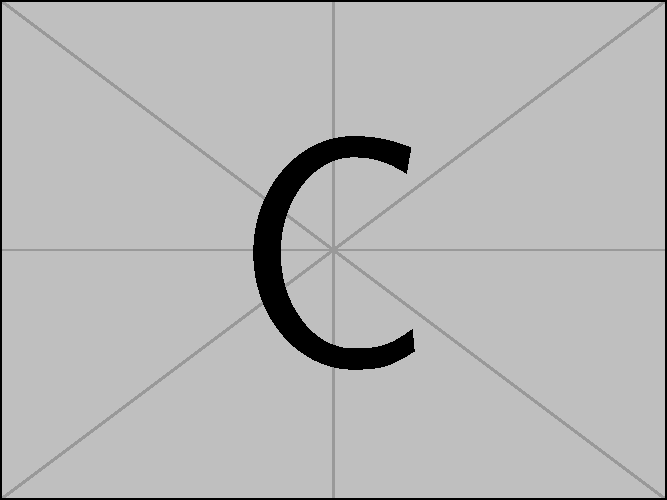
\includegraphics[width=0.162\textwidth]{example-image-c}
    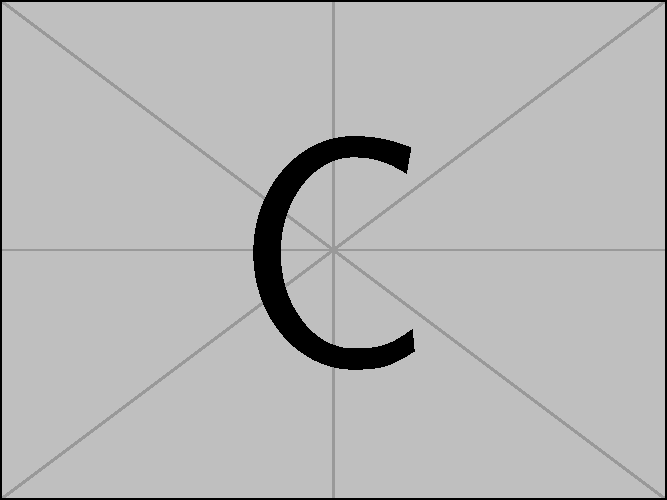
\includegraphics[width=0.162\textwidth]{example-image-c}
    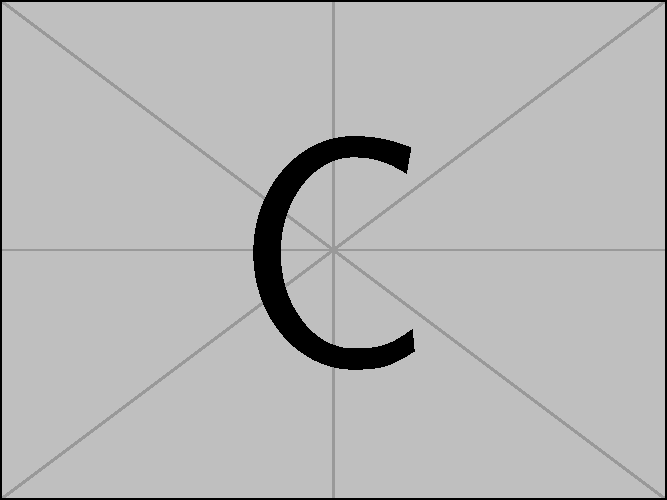
\includegraphics[width=0.162\textwidth]{example-image-c}
    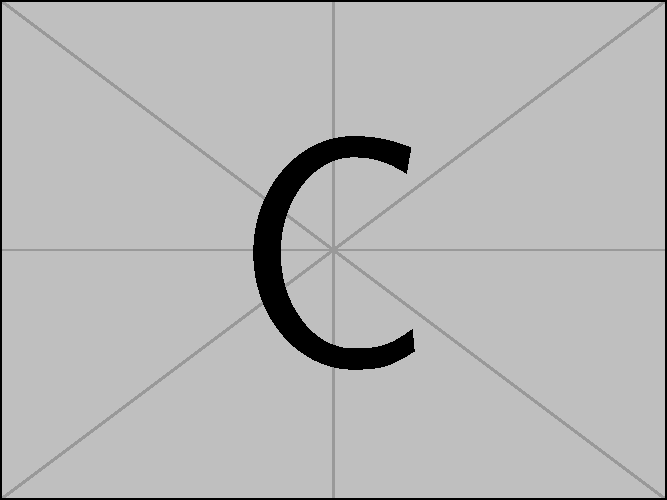
\includegraphics[width=0.162\textwidth]{example-image-c}
    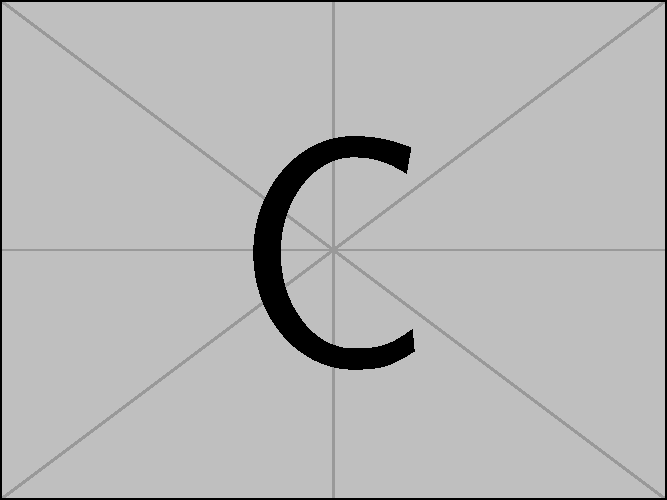
\includegraphics[width=0.162\textwidth]{example-image-c}
    \\
    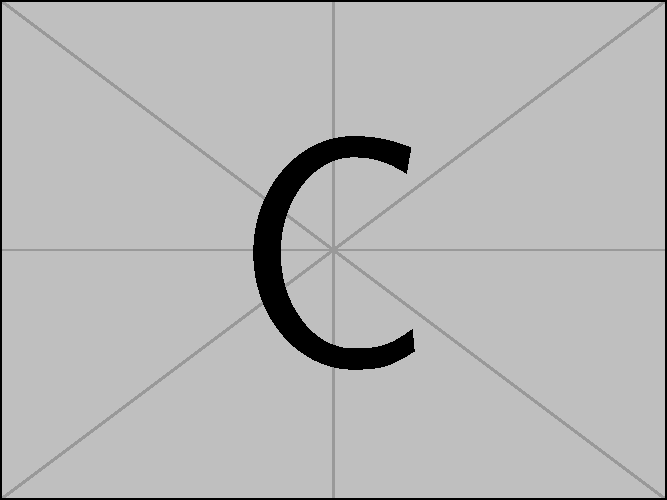
\includegraphics[width=0.162\textwidth]{example-image-c}
    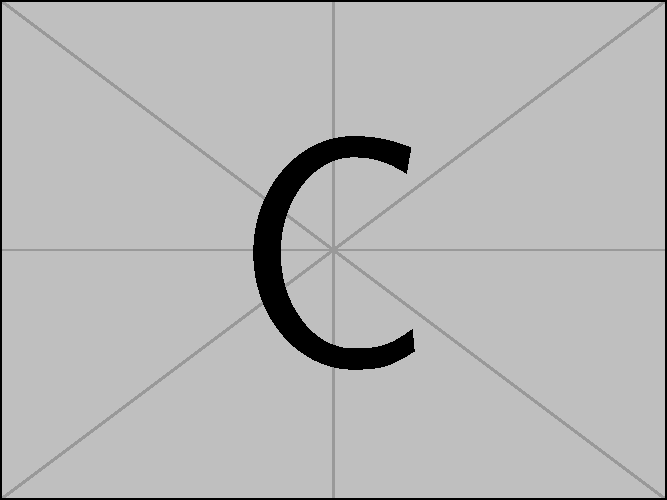
\includegraphics[width=0.162\textwidth]{example-image-c}
    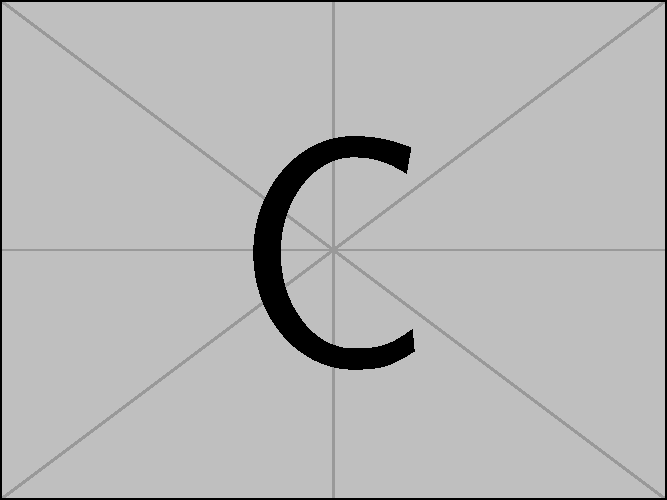
\includegraphics[width=0.162\textwidth]{example-image-c}
    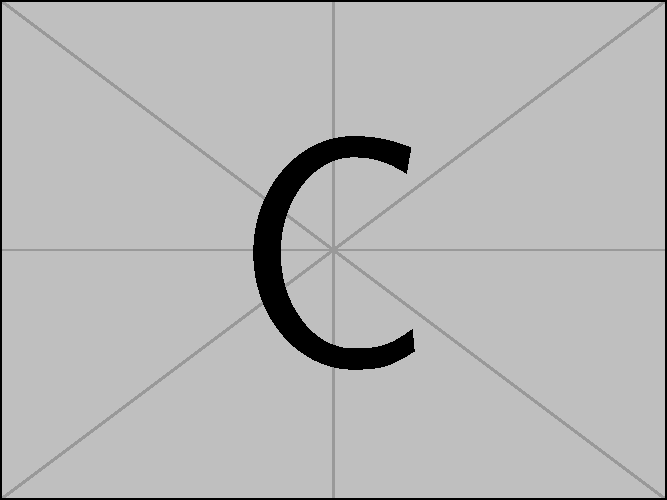
\includegraphics[width=0.162\textwidth]{example-image-c}
    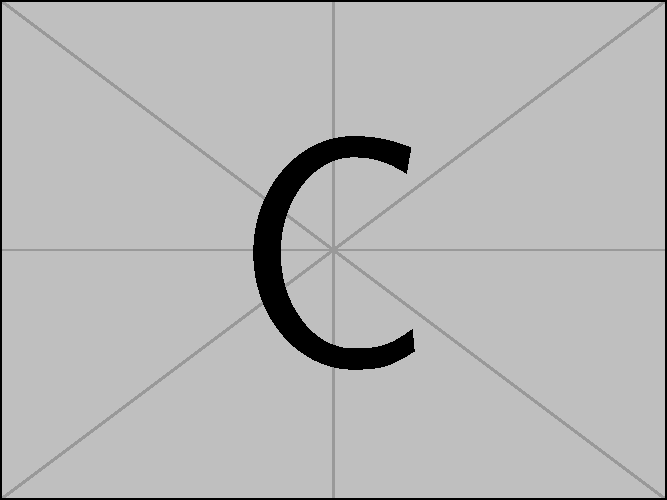
\includegraphics[width=0.162\textwidth]{example-image-c}
    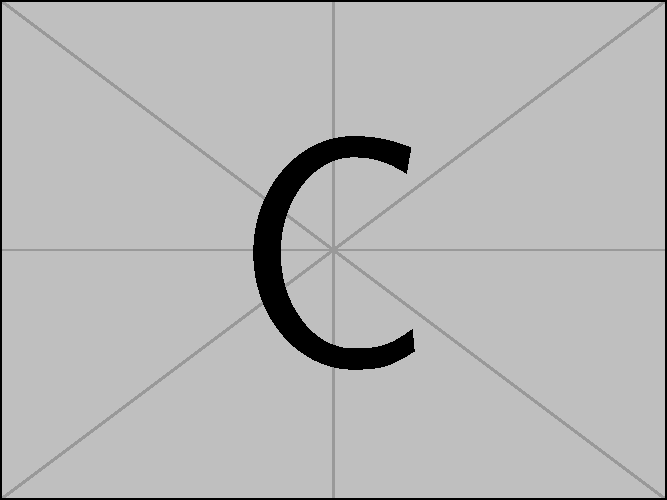
\includegraphics[width=0.162\textwidth]{example-image-c}
    \\
    \caption{A figure with multi-level images.} 
    \label{fig:fig10}
\end{figure*}
